\chapter{Indledning}
Vi har i dette projekt arbejdet med design og udvikling af et blodtryks målesystem. Ideen bag vores system blev udtænkt og udarbejdet med viden om en blodtryksmåler på en operationsstue på Herning Sygehus. Vores opstillede krav samt design til systemet, blev derfor lavet ud fra de oplysninger vi fik af en sygeplejerske\footnote{Anæstesi sygeplejerske Charlotte Høj, Herning Sygehus} på Herning Sygehus. Vi ønskede altså at lave et blodtryksmålersystem, som er så virkelighedsnært som muligt. Det design og de funktionaliteter vi efterstræbte at få opfyldt i vores projekt var derfor EKG, systoliske samt diastoliske blodtryk og iltmætning i blodet. Dette ønskede vi at få implementeret og hermed få grafer og værdier vist på en brugergrænseflade, som lever op til de standarder der ses på operationsstuer i dag. \\
\\
Baggrunden for dette projekt er, at man i klinisk praksis har behov for kontinuert at observerer patientens blodtryk. Det er i særdeleshed på intensiv afdelinger og operationsstuer, at man ønsker at lave invasiv blodtryksmåling. Ved invasiv blodtryksmåling kan man monitorere patientens fysiske tilstand under eksempelvis operation. Blodtrykket kan give en identifikation af blødning, smerter og hvor dybt patienten sover under narkosen. Denne overvågning giver det sundhedsfaglige personale en ekstra tryghed og sikkerhed om patientens tilstand under operation. \\
\\
Denne projekt rapport vil give en kort beskrivelse af vores samlede system samt krav hertil. Der vil være en udspecificeret projektbeskrivelse, som vil give et indblik i vores vej frem til det endelige resultat, og som også vil beskrive både de til- og fravalg vi har måttet tage, for at nå frem til netop det system vi ønskede at realiserer og præsenterer. Der har i den forbindelse været nogle ideer og ønsker, som ikke har været realistiske og tidsmæssigt mulige at opfylde og vil derfor være beskrevet i fremtidigt arbejde. Slutteligt vil derfor være en samlet konklusion på projektarbejdet.
\chapter{Projektformulering og afgrænsning}
\section{Oversigt over projektdeltagere og hovedansvarsområder}
Vi har i dette projekt valgt at dele projektets deltagerer op i to grupper med hver deres hovedansvarsområder. En som har beskæftiget sig med hardware og en som har beskæftiget sig med software. Derudover valgte vi i starten af forløbet at udvælge en projektleder, hvis opgaver bestod i at lave dagsorden for hvert møde, sørge for at deadlines blev overholdt, træffe endelige beslutninger og holde et overordnet overblik over projektet. Vi valgte også en procesleder hvis opgaver bestod i opgavestyring, godt arbejdsmiljø i gruppen og planlægning af projektforløbet. \\
Herunder ses de forskellige gruppemedlemmers hovedområde.\\\\
\begin{tabular}{| l | l |} \hline
\textbf{Hardware} & \textbf{Software}\\\hline
Brian Hansen & Ida Mark Skovbjerg \\\hline 
Mohamed Hussein Mohamed & Mette Østergård Knudsen \\\hline
Khaled Edwan & Line Skov Larsen  \\\hline 
\end{tabular}
\\\\
Under projektforløbet valgte vi at ændre denne rollefordeling, idet den generelle arbejdsfordeling samt arbejdsindsats i gruppen ikke fungerede optimalt. Vi valgte, at kun et gruppemedlem skulle varetage rollen som projektleder og procesleder, men at opgaver herunder kunne uddelegeres hvis nødvendigt. Denne leder blev i fællesskab valgt og baggrunden for dette valg var, at vi ønskede en leder som både havde viden og indflydelse på hardware og software, samt kunne træde i kræft hvis gruppearbejdet og deltagernes indsat ikke opfyldte den forventningsafstemning, som står skrevet i vores samarbejdskontrakt. Gruppens medlemmer med fulde navn og initialer ses herunder, det er initialerne benyttes som reference til gruppemedlemmerne herfra. \\\\
\begin{tabular}{| l | l |} \hline
\textbf{Fulde navn} & \textbf{Initialer}\\\hline
Ida Mark Skovbjerg & IMS \\\hline 
Line Skov Larsen & LL \\\hline
Mette Østergård Knudsen & MK  \\\hline 
Brian Hansen & BH \\\hline
Mohamed Hussein Mohamed & MM \\\hline 
Khaled Edwan & KE \\\hline
\end{tabular}
\chapter{Hjertet - en muskel}
Hjertet er en muskel, der fungere som en pumpe i kroppen. Hjertet pumper det iltede blod ud til resten af kroppen gennem arterie- og vene systemer. Når blodet passere ud af hjertet igennem arterierne sker der et tryk mod arterievæggene, dette kaldes blodtrykket. \\\\
Hjertet opdeles i to adskilte hjertehalvdele, som fungere som pumper. Den venstre, som pumper blodet rundt i organismen og den højre, som pumper blodet gennem lungerne. De to hjertehalvdele er sammensat af atrium og ventrikler. Det venøse blod føres tilbage til højre atrie gennem øvre og nedre hulvene. Mellem højre atrium og højre ventrikel sidder trikuspidalklappen, som forhindrer blodet i at løbe tilbage til atriet under hjertets sammentrækning. Fra højre ventrikel udløber i lungepuslåren, som deles ud i hver lunge. Mellem ventriklen  og lungepulsåren er pulmonalklappen, som forhindrer blodet i tilbageløb. I lungerne afgiver blodet CO2 og optager ilt. Det nu iltrige blod returneres gennem lungevenerne til venstre atrie. Fra venstre atrie til venstre ventrikel sidder mitralklappen. Fra venstre ventrikel pumpes blodet ud i aorta gennem aorta klappen, herfra pumpes blodet rundt i resten af organismen. \cite{hjertedsd}
\begin{figure}[H]
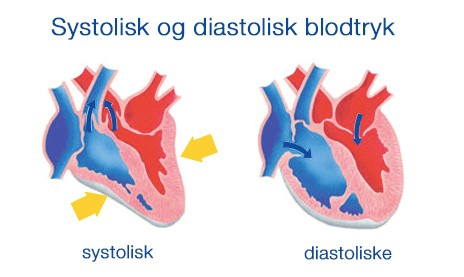
\includegraphics[width =0.5\textwidth , center]{billeder/sysdia}
\caption{\textbf{Her ses det systoliske og diastoliske blodtryk, og hvordan dette ses på hjertet}}
\end{figure}
\section{Blodtryk}
Blodtrykket er trykket i blodkarrene, når blodet pumpes rundt i kroppen. Dette tryk sker, når hjertets venstre hjertekammer trækker sig sammen og der, som resultat heraf, bliver presset blod ud i arterierne. Trykket vil altså være størst i arterierne, da arterierne er de blodåre som føres væk fra hjertet. Det laveste blodtryk vil være at se i venerne, da det er de blodårer som fører blodet tilbage til hjertet. Blodtrykket vises som to værdier: systolen, som er hjertets sammentrækningsfase og diastolen som er hjertets afslapningsfase. \\\\
Systolen angives som den kraft, der skabes når der kommer pres på karvæggen i arterierne. Dette sker i hjertets sammentrækningsfase, hvor blodet pumpes ud i arterierne. Systolen i et normalt blodtryk i hvile vil ligge i intervallet 100-140mm Hg og ved forhøjet blodtryk er værdien for trykket over 140 mm Hg. Diastolen angiver hjertets hvilefase og ses mellem to sammentrækninger. I denne fase fyldes ventriklerne med blod. Den normale værdi for diastolen ligger i intervallet 60-90 mm Hg. Hvis den overstiger 90 mm Hg anses blodtrykket for at være forhøjet. Udover systolen og diastolen kan også middeltrykket angives. Denne udregnes ved $\dfrac{2}{3}\cdot Diastole + \dfrac{1}{3}\cdot Systole$ \cite{blodtrykwiki}
Hypertension defineres som forhøjet systole, forhøjet diastole eller både forhøjet systole og diastole. Hypertension belaster hjertet, og medføre en øget risiko for udviklingen af apopleksi. Det er også forbundet med flere medicinske tilstande såsom arteriosklerose, hjerteinsufficiens og nyreskader. \cite{pulmonal} \\\\
Ser man på anatomien bag blodtrykket og blodtryksændring, ser vi på kredsløbssystemet, som omfatter blodets kredsløb, hjertet og lymfesystemet. Blodkredsløbet er et langt netværk af arterier og vener, som har til opgave at føre iltet blod ud til hver celle i kroppen, samt opfange affaldsprodukter fra celler og væv.\cite{pulmonal}  I lungekredsløbet udskilles affaldsprodukter og blodet iltes. Det er hjertet der pumper blodet ud i dette netværk, så blodet hele tiden er i bevægelse. Arterierne transportere blodet væk fra hjertet, og venernes opgave er at transportere blodet mod hjertet. 
\begin{figure}[H]
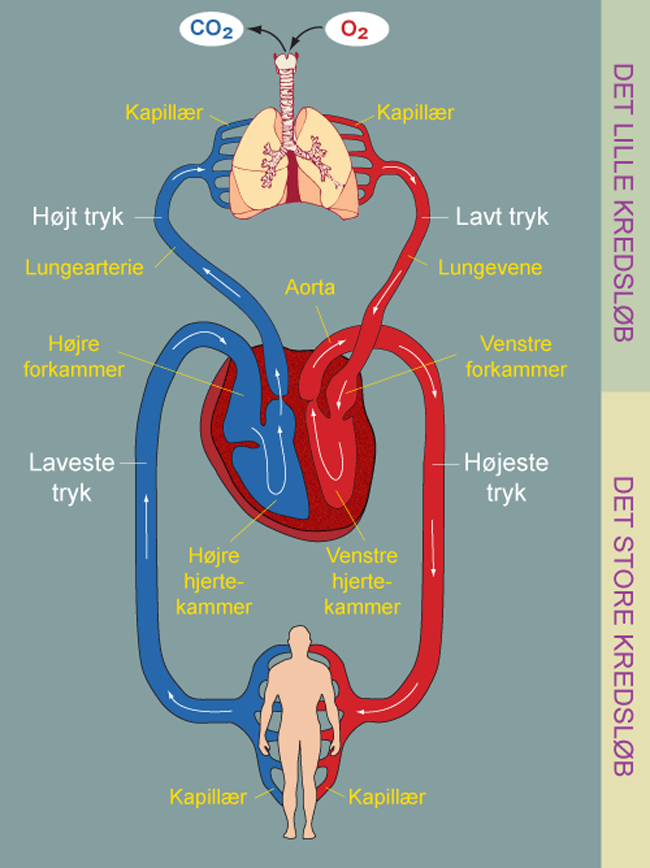
\includegraphics[width =0.5\textwidth , center]{billeder/hjertet}
\caption{\textbf{Det lille og det store kredsløb. Motoren der driver det hele er hjertet. \cite{hjertet}}}
\end{figure}
Kredsløbet kan funktionelt og anatomisk inddeles i to dele: Det pulmonale kredsløb og det systemiske kredsløb.
De to kredsløb fungerer i symbiose mellem hjertets højre hjerte kamre og hjertets venstre hjertekamre. Højre siden pumper blodet gennem det pulmonale kredsløb, og venstre side pumper blodet rundt i det systemiske kredsløb.
Det pulmonale kredsløbs primære funktion er at levere blodet til lungekredsløbet hvor blodet iltes. Hjertets højre side modtager iltfattigt blod og CO$_{2}$-rigt blod via v. Cava superior og inferior fra det systemiske kredsløb og pumper det videre ind i lungekredsløbet gennem det pulmonale kredsløb via pulmonal aterierne. Fra lungerne løber det nu iltrige og CO$_{2}$-fattige blod tilbage til venstre side af hjertet, som derfra pumper det videre til det systemiske kredsløb via aorta. \cite{pulmonal} 
\section{Direkte invasiv måling af blodtryk}
Den mest almindelig metode til klinisk at måle blodtryk er ved at koble det vaskulære tryk til en extravaskulær sensor via et væskefyldt kateter. Klinisk er dette systemet påsat patientens a. Radialies via en arteriekanyle. Kateterslangen er forbundet til en trevejs stophane og videre til tryk sensoren. Kateter-sensor systemet er fyldt med en saltvandsopløsning fra væskesøjlen. Denne saltvandsopløsning skal skylle cirka hvert andet minut gennem systemet, dette forhindrer blodet i at størkne på spidsen.
\begin{figure}[H]
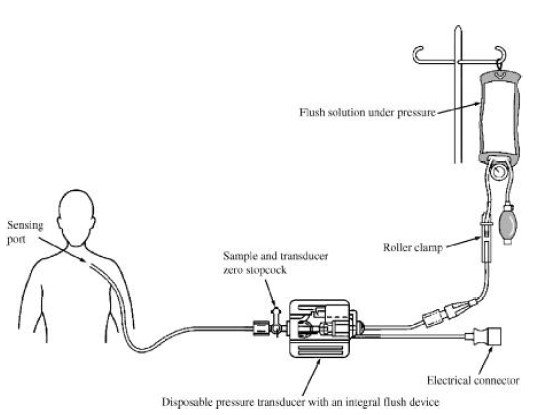
\includegraphics[width =0.7\textwidth , center]{billeder/kateter}
\caption{\textbf{}}
\end{figure}
Som det ses på figuren er sansningsporten indgangen til patients arterie. Kateteret er koblet til tre vejs stophanen og videre til sensoren. Tre vejs stophanen har tre mulige funktioner, 1: der kan lukkes for blodtilførslen så der er åbent for atmosfærisk luft og transduceren, dette giver værdien for nulpunktsjustering. 2: der kan åbnes for atmosfærisk tryk ind til blodåren, dette kan bruges hvis patienten skal have medicin. Her indsættes medicin og ved at åbne for trykket fra væskesøjlen, vil medicinen flyde med blodet ind i blodåren. 3: der åbnes for blodtilførsel ind i transduceren, dette giver blodtrykket. Blodtrykket transmitteres via kateter væskesøjlen ind i sensoren og til sidst i membranen. Det er her blodtrykket bliver målt. 
\chapter{Systembeskrivelse}
Det er blevet besluttet ud fra projektformuleringen at udvikle systemet som en prototype med perspektivering til fremtidigt arbejde. Forudsætninger for brug af systemet er at det skal køres på en computer samt overholde de opstillede krav. Systemet er opbygget af en hardwaredel og en softwaredel. \\\\
Hardwaredelen består af et aktivt 2. Ordens Butterworth Sallen-Key lavpasfilter, samt en forstærker. Forstærkeren modtager et signal fra den udleverede transducer, dette signal forstærkes op. Signalet sendes videre til lavpasfilteret hvor alle frekvenser over 50Hz bliver dæmpet. Her fra sendes signalet ind i dataopsamlingsenheden NI-DAQ.\\\\
Softwaredelen består af et window forms program udviklet i C\# .net, programmet skal kunne præsentere data indhentet fra DAQ’en. Ligeledes skal programmet kunne analysere og filtrere data fra DAQ’en, samt gemme disse i en "EPJ"-database. Programmet skal også kunne hente login-oplysninger fra en "personale"-database. \\
Man har valgt at have to databaser for at simulere det at der er en adskillelse af medarbejderdata og patientdata.
\begin{figure}[H]
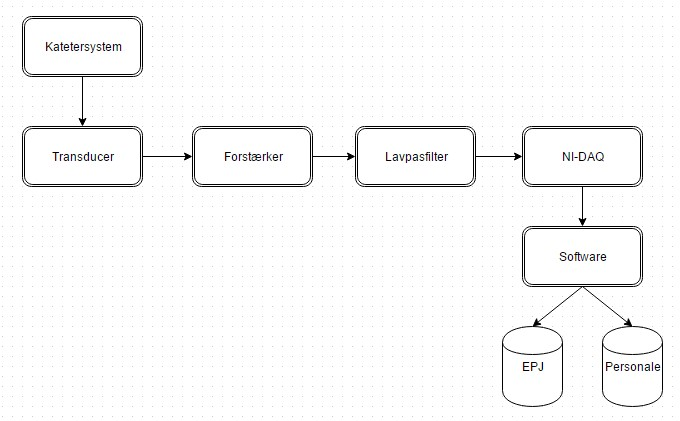
\includegraphics[width =0.8\textwidth , center]{billeder/system}
\caption{\textbf{Skitse af opbygning af systemet.}}
\end{figure}
\chapter{Krav}
Hvilke krav der stilles til produktet udarbejdes i en kravspecifikation. Denne kravspecifikation består af en række Use cases. Disse Use cases beskriver interaktionen mellem aktørerne og systemet. Use casene har til formål at specificere, hvilke krav der stilles til produktet. Kravene opstilles ud fra hvad kunden ønsker samt hvad leverandøren finder muligt at realisere. \\ \\
Der er nogle obligatoriske krav til produktet, der skal opfyldes. Disse krav er bl.a at systemet skal kunne kalibrere blodtrykssignalet og foretage en nulpunkts justering. Desuden skal blodtrykssignalet vises kontinuerligt, hvilket betyder, at signalet skal vises grafisk samtidigt med at det bliver hentet/indsendt fra hardwaren. Disse målte data skal efter de er blevet behandlet gemmes i en database.\\
Et af de obligatoriske krav er desuden at der skal være et digitalt filter der kan tilgås når programmet kører. Dette filter skal både kunne slås til og fra. Dette filter skal sørge for at signalet haves i to forskellige modes; et diagnose mode, hvor signalet er råt med alle udsving, og et monitor mode, hvor signalet er filtreret og afrundet.\\\\
Foruden disse obligatoriske krav er det valgt, at det skal være muligt starte og stoppe målingen. Når målingen er startet skal det være muligt at kunne justere grænseværdierne for systolen og diastolen, så disse værdier kan tilpasses. Når signalets værdier så kommer over grænseværdien, skal en alarmering begynde. Denne alarm skal kunne udsættes i et minut, dog kun alarmens lyd, så værdien blinker fortsat, så det stadig er tydeligt hvilken grænseværdi der er overskredet.\\
Systemet består af en computer med en programkode, en NI-DAQ, et lavpas filter, en forstærker, en transducer og en væskesøjle.
Systemet gør det muligt at få arterietrykket sendt ind i systemet igennem hardwaren. Arterietrykket dannes i denne prototype af en væskesøjle, som levere et tryk til en transducer, herefter sender transduceren signalet videre til hardwaren, hvor et lavpasfilter, filtrerer signalet, hvorefter en forstærker forstærker signalet. Dette signal sendes derefter igennem NI-DAQ ind i systemet, som derefter behandler og analyserer signalet.\\
Den fulde beskrivelse af de udarbejdede Use cases (fully dressed Use case skema) findes i dokumentationen under Kravspecifikation.
\begin{figure}[H]
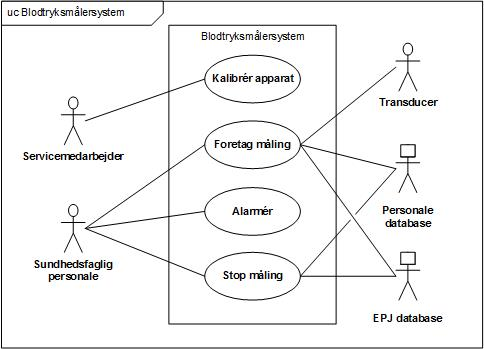
\includegraphics[width =0.7\textwidth , center]{billeder/UseCaseDiagram}
\caption{Use Case diagram. Dette diagram viser aktørernes interaktion med systemet.}
\end{figure}
\section{Aktørbeskrivelse}
Ud fra use case diagrammet ses de seks aktører; \textit{Sundhedsfaglig personale}, \textit{Transducer}, \textit{EKG patient}, \textit{EPJ database}, \textit{Personale database} og \textit{Servicemedarbejder}. Det er disse aktører der interagerer med systemet.
\subsection{Sundhedsfaglig personale}
Det er det sundhedsfaglige personale der er den aktør der påsætter måleudstyret på patienten. I dette tilfælde vil patienten være en transducer, hvilken er tilsluttet en væskesøjle. Det sundhedsfaglige personale er desuden den aktør der interagere med systemet; logger på og foretager en måling. Det sundhedsfaglige personale har dermed tilgang til de viste målinger på brugergrænsefladerne; startskærm og hovedskærm.
\subsection{Transducer}
Transduceren er i projektet den aktør der agere som patienten, denne består af en væskesøjle der er påsat en tryktransducer. Væskesøjlen levere et tryk i mmHg videre til tryktransduceren, og dette signal, der virker som arterietrykket, sendes videre i hardwaren, som behandler signalet. Derfor er denne aktør kilden til måleresultaterne for systole, diastole og middeltryk. 
\subsection{EKG-patient}
EKG patienten er den aktør som er kilden til EKG-kurven, idet vi ikke har en rigtig patient, hvorfra både EKG og blodtryk kan fås fra. Idet det er fra denne aktør at EKG-kurven findes er det fra denne aktør, pulsen kan bestemmes.\\
Værdierne for denne aktør hentes fra PhysioBank ATM.
\subsection{Servicemedarbejder}
Denne aktør, Servicemedarbejder, er den aktør, der står for at foretage kalibreringen. Dette gør Servicemedarbejderen ved at påsætte systemet til kalibrerings systemet, og indtaster de værdier for tryk (mmHg) og spænding (Volt), som måles ved tre forskellige målepunkter på en væskesøjle, hvorefter en kalibreringsværdi findes af systemet.
\subsection{EPJ database}
EPJ databasen, er databasen, hvori patientdata ligger samt den database hvori grafer og måleresultaterne, der bestemmes ved analysen, bliver gemt. Måleresultaterne er systole, diastole, middeltryk og pulsen.
Graferne for EKG-signalet og arteriekurven gemmes som tallister. Denne EPJ database skal simulere den database der fungerer på sygehusene i virkeligheden. Denne database kobler patienterne i denne database sammen med en sundhedsfaglig fra Personale databasen.
\subsection{Personale database}
Det sundhedsfaglige personales login informationer ligger i Personale databasen. Det er derfor denne database der indeholder informationer om det Sundhedsfaglige personale og dermed de informationer der benyttes til at tilgå systemet.
\section{Use case beskrivelse}
Use case diagrammet viser ligeledes de 4 Use cases der er for systemet: Kalibrér apparat, Foretag måling, Alamér og Stop måling. Disse Use cases er en beskrivelse af hvad systmet skal kunne og dermed beskriver de interaktioner der sker mellem aktørerne og systemet.
\\
\subsection{Use case 1: Kalibrér apparat}
Servicemedarbejderen skal i denne Use case foretage en kalibrering. Dette gøres ved at der er tre målepunkter på en væskesøjle, hvor en af disse vælges. På disse punkter måles spændingen (volt) og trykket (mmHg) aflæses fra væskesøjlen. Disse indtastes af Servicemedarbejderen ind i systemet igennem brugergrænsefladen; startskærmen. Herefter beregner systemet en kalibrerings værdi. Denne værdi bruges til at omskrive de indlæste værdier til en blodtrykskurve i mmHg.
\subsection{Use case 2: Foretag måling}
Denne Use case styrer målingerne af graferne der indhentes. For at dette kan gøres skal det Sundhedsfaglige personale først logge på systemet. Dette gør denne aktør ved at indtaste sit brugernavn og sin adgangskode på brugergrænsefladen; startskærmen. Når den sundhedsfaglige på logget på henter systemet de tilknyttede patienter, hvorefter det Sundhedsfaglige personale kan vælge den ønskede patient. Når Patienten er blevet valgt startes hovedskærmen, hvilken repræsenterer en blodtryksmålers brugergrænseflade. Her kan den Sundhedsfaglige starte målingen. Når dette gøres henter systemet arteriekurven og EKG-signalet. Dette bruges derefter af systemet til at beregne hhv. systole, diastole, middeltryk og puls. Systemet viser graferne kontinuerligt på hver sin graf og systole, diastole, middeltryk og puls vises som talværdier. Samtidig gemmer systemet automatisk kontinuerligt disse data i EPJ databasen. \\
Det vil være muligt for det Sundhedsfaglige personale at slå det digitale filter fra og til. Filteret er fra start slået til.\\
DEt er også muligt for det Sundhedsfaglige personale at justere grænseværdierne for systolen og diastolen, dette gøres for at indstille grænseværdierne mere individuelt for hver patient.\\
For at sikre at graferne der er hentet ligger rigtigt på graferne, kan det Sundhedsfaglige personale nulpunkts justere systemet, sådan at graferne kommer til at ligge rigtigt på akserne.
\subsection{Use case 3: Alarmér}
Alarmen startes af systemet, når en af grænseværdierne overskrides. Dette gør at grænseværdien der er overskredet blinker og at der starter en alarm lyd. Når alarmen kan endnu en grænse værdi overskrides, hvis dette sker begynder denne grænseværdi ligeledes at blinke, men der sker ikke noget med alarmlyden, denne fortsætter fra tidligere. \\
Det vil her være muligt for det Sundhedsfaglige af udsætte alarmen. Dette gøres ved at trykke på knappen, hvorefter at systemet stopper alarmens lyd i et minut, efter dette minut starter alarmens lyd igen. Grænseværdien/grænseværdierne der er overskredet fortsætter med at blinke indtil forholdene er normaliseret, altså indtil grænseværdien ikke længere er overskredet.
\subsection{Use case 4: Stop måling}
Det Sundhedsfaglige personale skal også stoppe målingen. Dette gøres ved at det Sundhedsfaglige personale interagere med hovedskærmen. Herefter vil det være muligt for det Sundhedsfaglige personale at logge 
\section{Ikke-funktionelle krav beskrivelse}
Ikke funktionelle krav er opsat efter FURPS+ metoden. Kravene er herefter blevet prioriteret efter MoSCoW.
\subsection{FURPS+}
\textbf{Functionality}\\
Funktionalitet er det brugeren ønsker sig. Dette omfatter også sikkerhedsrelaterede behov. Dette er krav til hvad programmet skal kunne af funktionalitet, f.eks. at programmet skal have et digitalt filter.\\\\
\textbf{Usability}\\
Hvor effektiv er produktet, set fra forbrugerens side, dette er det aspekt brugervenlighed ser på. Er produktet nemt at bruge. Hvordan bruges produktet; er der nogen brugergrænseflader. Det er herunder kravene til hvilke knapper der skal være på brugergrænsefladerne, og dermed også hvilke brugergrænseflader der skal være.\\\\
\textbf{Reliability}\\
Pålidelighed tager sig af aspekter som, hvor længe er det maksimalt at systemet må være nede. Er der fejl der kan forudses. Hvor præcist kan resultaterne vises. Er produktet let at vedligeholde; kan delene i produktet skiftes let.\\\\
\textbf{Performance}\\
Præstationen for produktet, handler om hvor hurtigt produktet er om at starte op og hvor hurtigt svartiden er. Hvor stor må svartiden maksimalt være. Så det er altså herunder, at det er beskrevet, hvor lang tid der går fra der er trykket på en knap, til at systemet svarer. \\\\
\textbf{S}uportability\\
Produktets support fortæller, om det er muligt at teste på produktet, om det er muligt at udvide produktet, installere og konfigurere produktet. Desuden om produktet er kompatibelt. Det er herunder programmets opbygnings model beskrives\\\\
\textbf{+}\\
Kunden kan have nogle yderligere behov, disse yderligere behov beskrives under +. Hvilke begrænsninger er der ved designet. Er der nogle krav for brugergrænsefladerne. Er der nogle fysiske eller implementerings krav. Er der dele der kan genbruges, herunder hele systemer eller dele af dem. Det er bl.a herunder at kravene til computeren der benyttes beskrives. \cite{furps}\\


\subsection{MoSCoW}
\textbf{Must}\\
De krav der bliver markeret som et must er de krav som produktet skal have. Altså det produktet skal have/indeholde.\\\\
\textbf{Should}\\
De krav der markeres som et should krav, er de krav til produktet der burde være med. Altså er det hvad produktet bør indeholde\\\\
\textbf{Could}\\
Kravene kan også markeres som could. Disse krav er de krav der kunne være gode at have med, men som ikke bliver prioriteret. Så det er kun, hvis man kan nu at få det med, at de skal være der.\\\\
\textbf{Would/Won't}\\
Det er ikke alle krav der skrives, der skal være gældende for produktet, disse krav markeres som would/won't. Det er altså disse krav som man ikke tager med eller de krav som ville være sjove at have med, men ikke har en betydning for produktet, men er en tilføjelse eller udvidelse. Det er disse krav der danner rammen for fremtidigt og videregående arbejde med projektet.
\chapter{Projektbeskrivelse}
\section{Projektgennemførelse}
\subsection{ASE-modellen}
Til udviklingen af dette produkt er der primært benyttet ASE-modellen. Modellen ses herunder. ASE-modellen er en udviklingsmodel, der er udarbejdet af Aarhus Ingeniørhøjskole. Denne model er en mellemvægtig semi-iterativ udviklingsproces, hvilken drives ud fra Use cases. Projektudviklerne fastlægger først en projektformulering, hvorfra en kravspecifikation kan udarbejdes, hvilke indeholder kravene fra kunden. Systemarkitekturen fastlægges ud fra kravspecifikationen, for derefter at designe og implementere de enkelte hardware og software dele hver for sig i iterationer. Til sidst fører dette til en accepttest, hvilken gennemføres, så der opstår een enighed mellem projektudviklerne og kunden.
\begin{figure}[H]
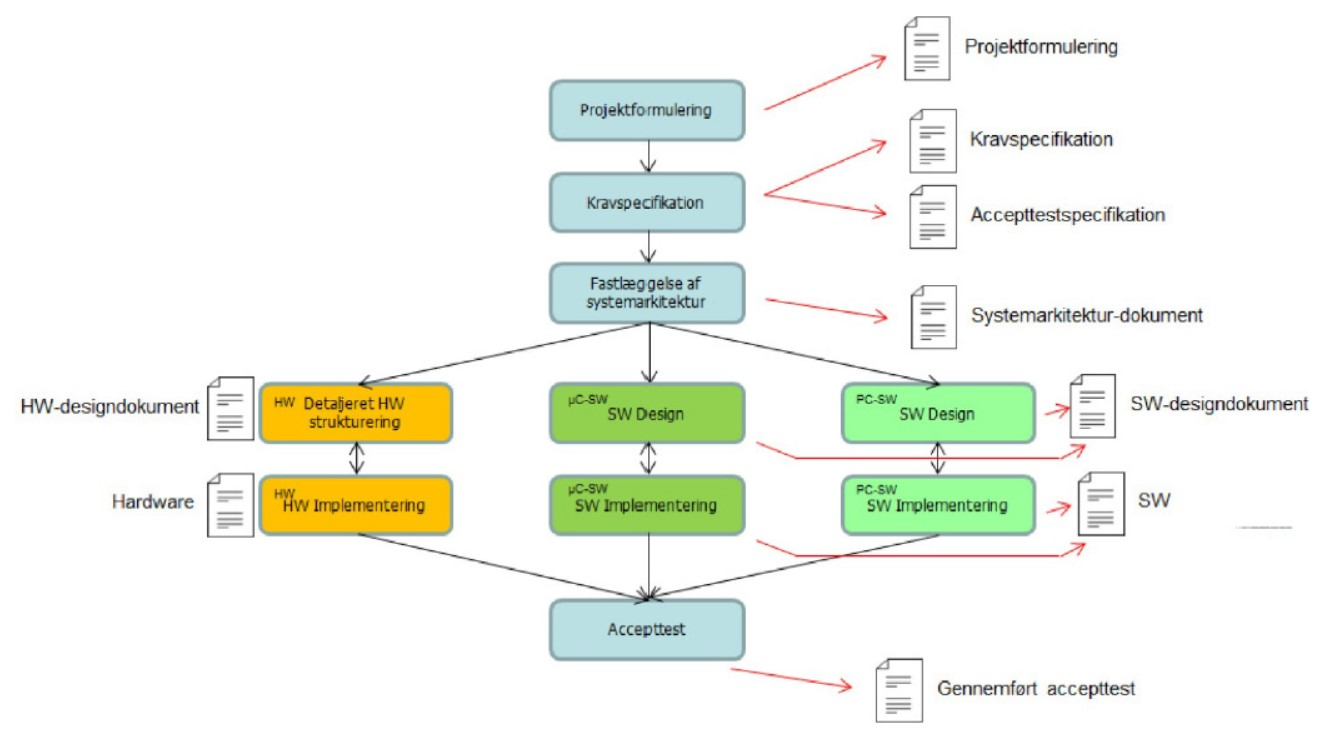
\includegraphics[width =1.0\textwidth , center]{billeder/ASEmodellen}
\caption{ASE-modellen.}
\end{figure} 
Kravspecifikationen bliver specificeret som en række Use cases ud fra problemformuleringen. Use cases benyttes til at beskrive aktørernes interaktion med systemet. Sammen med de ikke-funktionelle krav opnås der med Use casene et overblik over hvilke krav der stilles til systemets funktionalitet. Systemets design bestemmes igennem hardware og software design og implementering, herefter kan en accepttest udarbejdes. Ved udførelsen af accepttesten tjekkes det at kravene er opnået.
\subsection{V-modellen}
V-modellen en model som er faseopdelt udviklingsmodel. Denne model beskriver udviklingsfaserne og testfaserne i et projekt sideløbende. V-modellem er blevet benyttet sideløbende med ASE-modellen. Specifikationen af test foregår parallelt med udviklingen af selve systemet i V-modellen. Fordelen ved denne model er at testene sker på forskellige niveauer, hvilket sikre at udviklede delsystemer virker som ønsket. Det vigtige her er at en fase er færdiggjort, inden den næste fase påbegyndes. 
\begin{figure}[H]
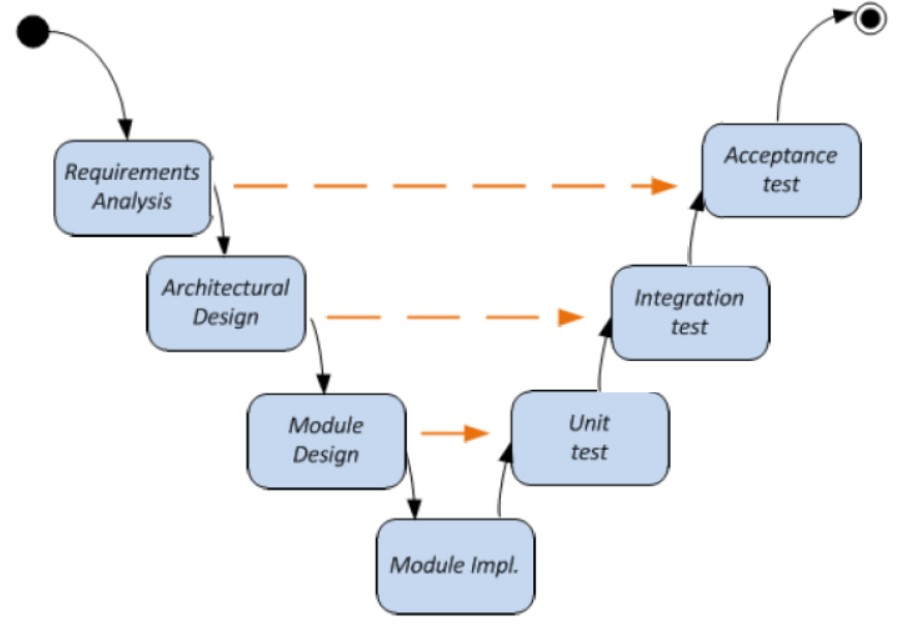
\includegraphics[width =0.7\textwidth , center]{billeder/Vmodel}
\caption{V-modellen.}
\end{figure} 
Ud fra modellen ses det at den første fase er udviklingen af kravspecifikationen. Her udarbejdes der en tilhørende accepttest, denne test gør det muligt at tjekke om systemet til sidst lever op til de opstillede krav. Den næste fase er herefter systemarkitektur, her udvikles den tilhørende test, denne test undersøger integrationen mellem de implementerede moduler. De sidste to fase af udviklingsfasen er design og implementering af systemets enkelte moduler, her udføres enhedstesten løbende af de implementerede moduler.
\subsection{Vandfaldsmodellen}
Vandfaldsmodellen er en model der bruges til udvikling af software, hvor softwareudviklingen betragtes som værende konstant løbende nedad. Her kan udviklingen af et modul i en ny fase først påbegyndes når den foranliggende fase er afsluttet. Denne model et i projektet benyttet til udviklingen af softwarearkitekturen. 
\begin{figure}[H]
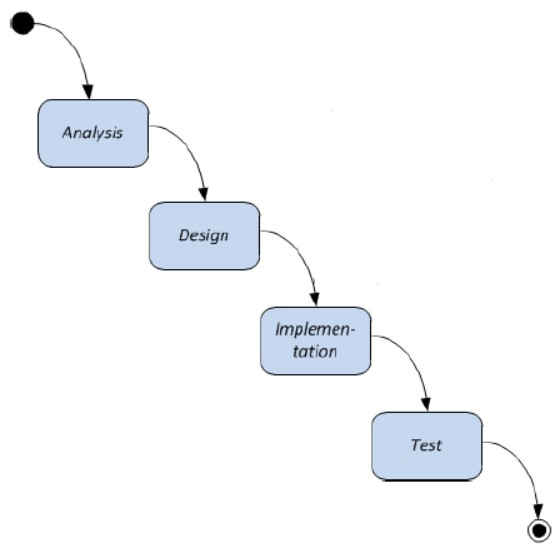
\includegraphics[width =0.5\textwidth , center]{billeder/Vandfald}
\caption{Vandfalds modellen.}
\end{figure} 
Disse tre modeller; ASE-modellen, V-modellen og vandfalds-modellen arbejder alle i en kronologisk logisk rækkefølge. Modellerne er benyttet i et omfang, hvor de har kunnet supplere hinanden. ASE-modellen giver det store overblik, mens V-modellen sikre udarbejdelsen af de nødvendige tests. Vandfalds-modellen er den proces, hvilken der er arbejdet ud fra i alle projektets facetter.   
\subsection{Projektstyring}
\subsubsection{Arbejdsfordeling}
Som nævnt tidligere valgte man fra projektets start at opdele gruppen i to hold, henholdsvis et softwarehold og et hardwarehold.
\subsubsection{Ændringer i projektstyring}
Under projektforløbet valgte vi at ændre denne rollefordeling, idet den generelle arbejdsfordeling samt arbejdsindsats i gruppen ikke fungerede optimalt. Vi valgte, at kun et gruppemedlem skulle varetage rollen som projektleder og procesleder, men at opgaver herunder kunne uddelegeres hvis nødvendigt. Denne leder blev i fællesskab valgt og baggrunden for dette valg var, at vi ønskede en leder som både havde viden og indflydelse på hardware og software, samt kunne træde i kræft hvis gruppearbejdet og deltagernes indsat ikke opfyldte den forventningsafstemning, som står skrevet i vores samarbejdskontrakt. 
\subsubsection{Scrum}
Det blev i øvrigt besluttet at benytte SCRUM som hjælp til styring af projektet. Der blev udnævnt en tovholder som skulle holde møder i løbet projektets udarbejdelse samt styre opgaverne. Man valgte at bruge Pivotal Tracker \cite{tracker}  til at styre og prioritere opgaver. Der var en overordnet tidsplan fra start, denne tidsplan består af en række deadlines – den kan findes i dokumentationen.
\subsubsection{GitHub}
Det blev besluttet at benytte Github til deling af informationer og dokumentation i forbindelse med udarbejdelse af rapporten. Det blev vurderet at det var vigtigt at der var en central informationsudveksling så begge grupper kunne følge med i hvor langt de var i de forskellige processer. 
\subsubsection{Iterativ udviklingsproces}
Udviklingsprocessen på både software- og hardware-holdet blev meget iterativ, det betød at der var mange forskellige versioner af både hardware og software. Man valgte denne metode da store dele af projektet var et teknologistudie, så det var nødvendigt at lave mange iterationer løbende. Desuden var det vigtigt at de to hold kunne omstille sig hurtigt, og drage ny viden til nytte uden at skulle igennem en langsommelig design proces på ny.
\section{Metode}
\cite{SysML} For at beskrive den overordnede systemarkitektur og det detaljerede design for produktet, er der blevet benyttet SysML og UML. SysML er et grafisk modelleringssprog, hvilket kan hjælpe til at forstå og udvikle selv komplekse systemer. SysML udspringer af UML, dog benyttes SysML i højere grad ved systemer, der både indeholder software og hardware, end UML. UML benyttes til at beskrive softwaresystemets struktur og forløb. \cite{uml}
\\
\\
SysML’s struktur-, funktionalitets og adfærdsdiagrammer er i projektet blevet benyttet til at specificere og dokumentere systemet og dets komponenter. Der anvendes to strukturdiagrammer; block definition diagram (BDD) og internal block definition diagram (IBD) for at vise systemstrukturen. Systemarkitekturen bliver delt op i blokke. BDD'et bruges til at vise forholdet mellem de forskellige blokke, deres komposition og forhodlet mellem logiske- og fysiske enheder i systemet. IBD'et benyttes til at vise den forbindelse der er imellem de forskellige blokke der ses ud fra BDD'et. Dermed ses den vej signalet går igennem de forskellige enheder og hvordan disse enheder er koblet sammen.\\
\\
For at kunne beskrive produktets funktionalitet er der blevet benyttet et Use case diagram. Dette diagram beskriver, hvordan systemet interagerer med de udefrakommende enheder (f.eks. aktører) for at løse et antal af opsatte opgaver. Disse opgaver er beskrevet i forskellige Use cases. Et af adfærdsdiagrammerne er et sekvensdiagram, denne viser de handlinger der er mellem systemets dele (parts), hvilke er delt op i sekvenser.\\
For at beskrive overgangen fra de beskrevne Use cases til software, er applikationsmodellen benyttet. Applikationsmodellen tager udgangspunkt i Use cases og domænemodellen, hvor Use cases bruges til at identificere, hvad systemet skal kunne og hvordan det skal løses. Domænemodellen beskriver det overordnede systemdomæne. Systemdomænet beskrives ud fra de konceptuelle klasser, hvilke findes ud fra Use cases. Domænemodellen definere de klasser der skal være i softwaren og de interaktioner der er imellem disse, dette gøres med klassediagrammer og adfærdsdiagrammer. \\
\\
En applikationsmodel med kontrolklasser, domæneklasser og boundaryklasser kan opbygges. Kontrolklasserne er funktionen at beskrive hvordan data behandles mellem domæne- og boundaryklasserne. Domæneklasserne indeholder funktionaliteten som det pågældende softwaremodul benytter, det er herfra klasserne der skal bruges i softwaren identificeres. Boundaryklasserne har den funktion at beskrive hvordan systemet kommunikerer med omverdenen og omvendt. Ved at benytte applikationsmodellen til design af softwarens opbygning gøres det lettere at udvikle et produkt med lav kobling samt høj samhørighed. \\
\\
Systemets softwarestruktur og forløb beskrives ved at benytte UML klassediagrammer. Disse klassediagrammer viser den struktur der er mellem et objektorienteret systemklasse, og kan derfor bruges til at definere relationen mellem de forskellige klasser. Derfor dannes der et hurtigt overblik over sammenhængen i systemet ved at benytte klassediagrammet.  
\section{Specifikation og analyse}
I det følgende afsnit beskrives de overvejelser der er gjort i projektet i forbindelse med specifikation og analyse af henholdsvis hardware og software delen. Gennem afsnittet startes der med at kigge på hvilke specifikationer der er valgt, analysen og grunden til dette. Afsnittet er inddelt i at først kigge på specifikations og analyse arbejdet angående det lavpasfilteret og operationsforstærkerne. Derefter vil der blive beskrevet specifikations og analyse arbejdet angående det digitale filter, udregning af blodtryksværdi og præsenter data på en pæn måde på et brugergrænseflade.
\subsection{Hardware}
En af de krav der var til Hardwaren givet fra projektets vejledning var, at der skulle designes et lavpas filter med en cut-off frekvens på 50 Hz. Et andet krav var at filteret skal kunne dæmpe med 40db pr. dekade ved 500 Hz. Der bliver desuden opgivet at kondensatoren C2 skulle have en værdi på 680 nF. \\
Der var også opgivet krav til filteret at det skulle være et anden ordens butterworth sallen key filter. Herved er der valgt. \\
Ud fra krav omkring filteret og værdien af kondensatoren, er der opstillet overføringsfunktionen for Salle-Key anden ordens filteret. Overføringsfunktionen er udformet ud fra vejledningen for det faglige indhold, som indeholdte de krav der var opgivet til projektet, fra skolen.
\begin{align}
\dfrac{V_{out}(s)}{V_{in}(s)}=\dfrac{\dfrac{1}{R1\cdot R2\cdot C1\cdot C2}}{s^2+\dfrac{R1+R2}{R1\cdot R2\cdot C2}\cdot s+\dfrac{1}{R1\cdot R2\cdot C1\cdot C2}}
\end{align}
Analysen af filteret er lavet, ved at omskrive overføringsformlen til en standard formel for anden ordens filtre. I standard formlen for anden ordens filtre, er der isoleret cut-off frekvensen, og opstillet en ligningfor denne. \\
Igennem arbejdet med analysen af filteret, blev der efter flere iterationer, fundet ud af at værdien for kondensatoren C1, skulle være det halve af C2. Da C2 også var en af kraven til projektet og var opgivet i vejledningen for projektet, kunne værdien for C1 udregnes til 340nf. Dette svare til det halve af C2 som er 680nF.\\
Da der nu er specificeret værdierne for begge kondensator og en ligning for cut-off frekvensen, som også er specificeret til 50 Hz, er de to modstande R1 og R2 udregnet. 
\begin{figure}[H]
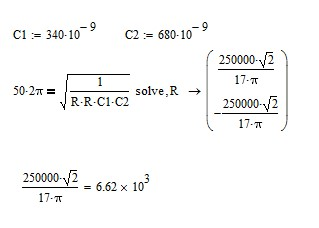
\includegraphics[width =0.3\textwidth , center]{billeder/mathcad2}
\caption{\textbf{Beregning fra Mathcad}}
\end{figure}
Der er nu specificeret alle komponent værdier for anden ordens butterworth sallen-key filteret. For at sikre sig at specifikationerne er sat til de rigtige værdier, er der lavet en analyse i matlab ved at lave et bodeplit over amplituden. På bodeplottet kigges derefter om grafen falder ved 50 Hz, og om der er faldet 40 db pr. dekade ved 500 Hz. Ud fra bodeplottet er der konkluderet at specifikationerne for filteret er rigtige, da grafen er faldet 3db ved 50 Hz. Der kan også aflæse fra grafen at filteret er faldet 40db pr dekade, dette ses ved at fra cut-off frekvensen på 50 Hz, går der en dekade før den er faldet til en amplitude 40 db, som svare til en frekvens på 500Hz. 
\begin{figure}[H]
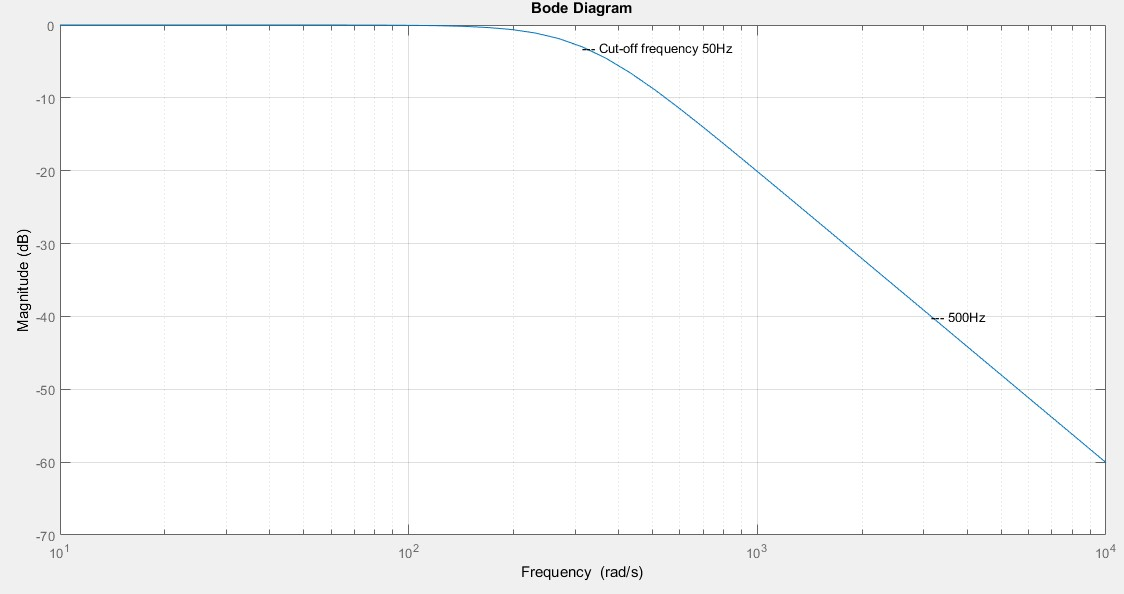
\includegraphics[width =0.6\textwidth , center]{billeder/bodeplot}
\caption{\textbf{Bodeplot}}
\end{figure}
Operationsforstærkeren For at kunne dimensionere operationsforstærkeren tilfredsstillende, kiggede man på de allerede forelagte krav samt hardwaredele der var til stede. Det elektriske signal fra tryktransduceren(TruWave\texttrademark) som skulle sendes i vores dataopsamlingsmodul (NI-DAQ6009), skulle således forstærkes i tilstrækkelig grad. Dette giver større præcision i vores målesignaler og mindre fejlmargin. Den maksimale spænding DAQ’en kunne tage imod er +/- 10V, det vil sige der ikke måtte forstærkes mere op en +/- 10V. Man valgte at benytte en INA114 efter anbefaling fra medstuderende og vejleder. Til forstærkeren valgte man to 9V-batterier som spændingsforsyning, dette ville give os teoretisk maksimal forstærkning på +/- 9V, da vi valgte at bygge spændingsforsyning op så den ville levere 18V peak-to-peak. Man sikrede sig ved hjælp af udregninger at båndbredden og den gain der kunne leveres var tilstrækkelig i INA114-forstærkeren. Ligeledes udregnede man størrelsen på den modstand der regulerer gain, det blev besluttet at benytte et potentiometer i stedet for en fast modstand for at imødekomme evt. udsving i forbindelse med opbygning på fumlebræt samt \%-tolerance i komponenter.
\subsection{Software}
I projektvejledningen var der opstillet krav omkring at softwaren skulle implementer digitalt filter, skulle kunne vise data kontinuert, kunne kalibrer og fortage en nulpunktsjustering, gemme data i enten en tekstfil eller database og det digitale filter skal kunne slås til og fra. \\
Der er implementeret et avearge moving filter, som tager summen af blodtrykstallene og sender videre. Efter snak med vejledere er der valgt et avearge moving filter. Fordelen ved dette filter er at der udglatter hver enkelt værdi for blodtrykket, i stedet for at udglatte få områder af blodtrykssignalet. Filteret bliver herefter ganget på alle værdierne for blodtrykket. Der er valgt dette filter fordi det kan bruges på et kontinuert signal, da det bare udregner summen på det den har fået ind, og udregner en ny sum ud for hvert tal. \\\\
Kravet om at kunne kalibrere er blevet specificeret ved at oprette en kalibreringskoefficient. Denne kalibrerings koefficient er fundet frem ud fra vandsøjlen, hvor der ved 50mmHg, gav et signal med 1 volt, herved er der udregnet at kalibrering koefficienten til 50. Denne kalibrerings koefficient er implementeret i software koden i en appconfig fil, som er en xml fil. Dette er valgt, for at hvis der ikke kalibreres hver gang, er der en default kalibreringsværdi som koden kalibrer efter. Herved kan sygeplejerskerne springe kalibrering over, og gå direkte til måling efter at have logget ind. Der skal kalibreres engang om året, herved er kalibrering indsat på StartGUI, hvor der kan indtastes mmHg og volt værdier, herefter udregner programmet kalibrerings koefficienten ved at divider disse to, og gemme dem som en lokal variable. \\\\
Kravet om at kunne vise en måling kontinuert er løst ved at bruge object stragy mønstret, hvor der er tilknyttet et subject til, som hele tiden giver besked om der er sket ændringer.  Object strategy er valgt, da det giver mulighed for at sende data imellem to klasser, hver gang der bliver indlæst nye tal af DAQ’en. Observer strategy er også valgt til at sende analyseret data fra logiklaget til præsentation oppe på brugergrænsefladen. For at vise data kontinuert er der lavet en kø og en update metode, som hele tiden opdater grafen op på brugergrænsefladen. Køen gør at der puttes en masse tal ind i en række, og præsenter det første tal der puttet ind i køen først, på brugergrænsefladen. \\\\
Efter analyse af dette mønstre er der vurderet at opbygge det efter push princippet, så hver gang der bliver indlæst et tal fra DAQ’en bliver dette tal via subjectklassen sendt videre til fra daqklassen til logiklaget. Dette sørge for at data bliver sendt op igennem programmets trelags struktur. \\\\
Til at gemme er specificeret to databaser, EPJ og Personale database. Der er valgt at bruge en patient database, da der skal kunne hentes et brugernavn og login for anæstesi sygeplejerske, der skal monitorere et blodtryk for en patient. Dette login sørger for at kun personalet kan have adgang til at bruge blodtryksmålersystemet.  Der er valgt at det skal være databaser, i stedet for at en fil, da der skal kunne ligges data i og hentes filter fra databasen fra forskellige computere og servere. Der valgt at snakke sammen med EPJ database, for at hente informationer om den patient der måles på. Informationer om patienten er vigtig, for at se om deres eventuelle sygdomme, og gamle blodtryksmålinger, for at kunne diagnosticere nuværende anormaliteter og grunden dertil. Patientens navn og cpr bliver vist på Hovedskærmen. \\\\
Nulpunktsjutering er et krav der et opgivet i projektvejledningen. Efter snak med vejleder er der specificeret at nulpunktsjustering skal ske efter at signalet er indlæst af DAQ’en. Der er analyseret frem til at der skal nulpunktsjusteres for det atmosfæriske tryk der kommer igennem transduceren. Der er efter videre analyse kommet frem til at det atmosfæriske tryk er en ret linje. Der er specificeret til at gøre dette ved at manuelt måle det atmosfæriske tryk ved at åbne op for transduceren, så der måles det atmosfæriske tryk, som er tilkoblet det analog anden ordens filter og operationsforstærkeren og måle igennem programmet Waveform, hvilke data der bliver opsamlet af DAQ’en. Da det er en ret linje, aflæses der kun en værdi i volt. Denne værdi indskrives på brugergrænsefladen på HovedGUI, og der skal trykke nulpunktsjustering. Der specificeret at nulpunktsjusteringsværdien ganges på alle blodtrykstallene inden de bliver vist i grafen. Det er valgt for at undgå større ændringer af blodtrykssignalet, når det er vidst på grafen. 

	\section{Arkitektur}
	\subsection{Hardware}
	kort indledning
	Hardware beskrivelse
	Signalets vej
	BDD/IBD indsættes
	\subsection{Software}
Systemets softwarearkitektur beskrives på baggrund systembeskrivelsen og kravspecifikationen. Ud fra relevante diagrammer og modeller kan software beskrives hvorfra arkitekturen for softwaren opnås. Samtlige diagrammer og modeller kan findes i Projektdokumentationen under Arkitektur og design.
\subsubsection{Problemidentifikation}
Først skulle det identificeres hvad produktet skulle bruges til og hvordan det skulle virke. Her blev der i først omgang ud arbejdet en idé til at produktet skulle benyttes ved blodtryksmåling på diabetes patienter. Dette førte til at der blev lavet en startskærm, hvorfra det kunne vælges, hvor målingen skulle foretages, sådan at data efterfølgende kunne analyseres. Dette skulle føre til en diagnosticering af hvor slem diabetes patienten havde og dermed hvor lavt blodtrykket er ude i underekstremiteterne. Denne idé blev dog kasseret, da det blev klargjort at foretage en invasiv i underekstremiteterne, på en diabetes patient, hvor dette ikke vides præcist hvor lavt blodtrykket er i underekstremiteterne, ville være en rigtig dårlig idé. Dette er den, da en direkte invasiv blodtryksmåling foregår ved at systemet påsættes patienten via en arteriekanyle. Da en diabetes patient har lavere blodtryk i underekstremiteterne og dermed dårligere blodstrømning, vil det ikke være smart at påsætte en arteriekanyle, dette vil kunne resultere i en infektion. En ny idé blev derfor udarbejdet. Her skal produktet ligne en blodtryksmåler der fungerer på sygehusene. Derfor blev et møde med anæstesi sygeplejerske Charlotte Høj fra Herning sygehus afholdt. Her blev et blodtryksmålingsscenarie vist. På EPJ-systemet (EPJ-computer) skulle man først logge på, hvor patienten på hvem målingen skulle foretages kunne vælges. Herefter kunne blodtryksmålingen foretages på patienten. Denne idé blev dermed idéen til projektet.\\\\
Ud fra denne idé kunne Use cases udarbejdes, disse er beskrevet under Krav, hvor hovedscenariet for brugen af blodtryksmåleren beskrives.
\subsubsection{Domænemodel} 
Ud fra disse Use cases kunne de klasse som systemet skulle bestå af identificeres. Disse klasse identificeres ved at bestemme de konceptuelle klasse, som indeholder den information som systemet skal holde styr på. De konceptuelle klasse indføres i domænemodellen som klasser. Det er i domænemodellen hvor problemet i forhold til hvad der skal holdes styr på i softwaren kan bestemmes. 
\begin{figure}[H]
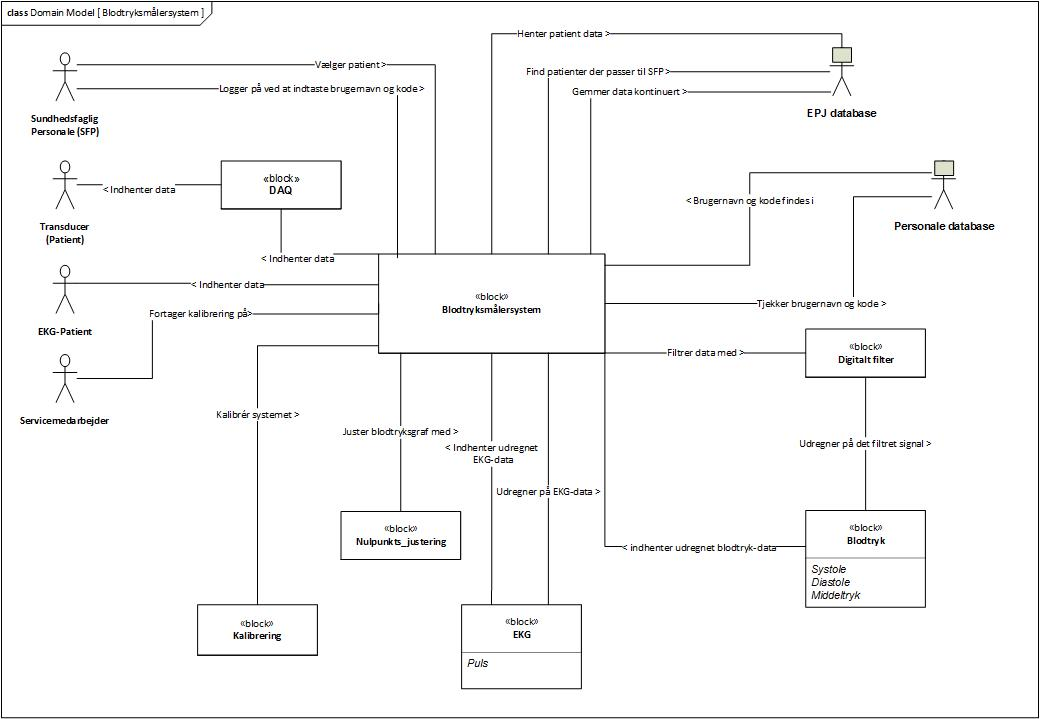
\includegraphics[width =1.0\textwidth , center]{billeder/DM}
\caption{\textbf{Domænemodel for blodtryksmålersystemet.}}
\end{figure}
Ud fra denne model ses det sundhedsfaglige personales interaktion med systemet, samt hvilke handlinger der igangsættes af denne interaktion. Det sundhedsfaglige personale udfører en handling, der medfører, at en række processer starter i systemet. Disse processer sørger for
at hente data fra transduceren og EKG patient, samt sørger for at starte beregningen af værdierne for puls,
systole, diastole og middeltryk. Efter beregningerne viser systemet disse værdier på brugergrænsefladen, samt sørger for at disse data bliver gemt i EPJ database. 
\subsubsection{Klasseidentifikation}
Ud fra domænemodellen kan softwareklasserne altså identificeres. Dette fører til at en applikationsmodel kan opstilles. Applikationsmodellen bruges til at bestemme de interagerende klasse i blodtryksmålersystemet og hvordan disse klasser kan tale sammen. Det er altså også ud fra applikationsmodellen at det kan bestemmes, hvilke klasser der skal ligge i de forskellige lag i trelagsmodellen, da klasserne i applikationsmodellen kan være af typen; domain, doundary og control.\\\\ Controlklasserne (kontrolklasserne) er de klasser er udfører Use casene ved at interagere med domai- og boundary klasserne. Boundaryklasserne (grænseklasserne) er de klasser der repræsenterer aktørerne fra Use Casene og disse aktøreres grænseflader. Domainklasserne (domæneklasserne) er de klasser hvori data bliver behandlet og bearbejdet. Domæneklasserne er de klasser der skal ligge i logiklaget. Præsentationslaget og datalaget indeholder begge boundaryklasserne, det skal derfor identificeres hvilke indeholder data og hvilke klasser hvorfra interaktionerne startes.
\subsubsection{Metodeidentifikation}
Ud fra klasserne identificeret af domænemodellen og applikationsmodellen, kan sekvensdiagrammer laves. Sekvensdiagrammerne er interaktionsdiagrammer og viser derfor hvordan processerne forløber i forhold til hinanden. Der laves et sekvensdiagram for hver Use case. Ud fra sekvensdiagrammerne kan det altså ses hvornår og hvordan de forskellige processer forløber i systemet og interagerer med hinanden. Softwaremetoderne kan derfor identificeres ud fra sekvensdiagrammerne.\\ 
Ud fra sekvensdiagrammerne kan et klassediagram laves. Dette diagram viser hver metode og attribut i hver klasse.
\section{Design, implementering og test}
\subsection{Software}
Ud fra arkitekturen kan designet af softwaren bestemmes. Det bestemmes hvilke mønstre der skal benyttes og hvordan data skal transporteres igennem koden.
\subsubsection{Observer mønsteret}
Observer/subject mønstreret bruges til at sende data op kontinueret og på en fornuftig måde. Subject har en metode til at koble en obeserver til, og en anden metode til at fjerne observeren. Der er en tredje metode i subject, kaldet notify. Notify sørger for at give besked til den tilknyttet observer om opdatering. En observer er interesseret i at kende til ændring i et objekt. Beskeden om ændring kommer fra subjectet, der er tilknyttet observeren. \\
\\
I dette projekt er der valgt at bruge observer/subject mønstreret til at sende data fra datalag til logiklaget. Mønstreret er også brugt til at sende data videre fra logiklaget til præsentationslaget. Yderligere beskrivelse findes i projektdokumentationen under kapitlet Arkitektur og design under afsnittet Software design. 
\subsubsection{PUSH/PULL}
PUSH/PULL er et software mønstre, der enten skubber eller trækker data op. PUSH betyder at skubbe, og betyder at data bliver skubbet op, når der sker en ændring, uden der skal gives besked om at hente data. PULL trækker data op imellem lagene. I PULL gives der besked til et lag om en ændring. Herefter skal laget der ønsker at kende til ændringen bede om ændringen, før det sendes op.\\
\\
I dette projekt er der valgt PUSH mønstret, da det er interessant at få målinger op til brugergrænsefalden hele tiden når, er indlæst nye målinger fra DAQ’en, og få sendte målingerne sammen med. Yderligere beskrivelse findes i projektdokumentationen under kapitlet Arkitektur og design under afsnittet Software design. 
\subsubsection{Queue}
For at sikre at data bliver sendt op i den rigtige rækkefølge og på en kontrolleret måde, er der i dette projekt valgt at benytte en kø. Til dette er der benyttet en indbygget funktion i Visual Studio, Queue class. Herunder ligger der to metoder, som kan bruges til at sende objekter af tal ind i den ene ende af køen og efter at køen er blevet fyldt op, er der en funktion til at fjerne det første objekt fra den anden ende af køen. Dette sørger for at der hele tiden er et flow i køen når der sendes data ind i denne. \\
\\
En yderligere beskrivelse af hvordan Queue klassen benyttes i koden og hvordan denne er opbygget er beskrevet i dokumentationen under Arkitektur og design under afsnittet Implementering.
\subsubsection{Trelagsmodel}
Trelagsmodellen er en software model, til at inddele sin software i tre lag, præsentationslaget, logiklaget og datalaget. Hver lag har sit eget ansvar og funktionalitet. Præsentationslaget kan kun tilgå logiklaget, og må kun vise data på brugergrænseflade eller indlæse data fra brugergrænsefladen. Logiklaget må tilgå både datalaget og præsentationslaget. Logik er det midterste lag, og står for behandling af data fra præsentationslaget og datalaget. Datalaget er det nederste lag og sørge for at sende data fra et måle apparat op til logiklaget. Datalaget står også for at gemme data i en fil eller en database.\\
\\ 
I dette projekt er koden opdelt efter trelagsmodellen, ved at have et præsentationslag med to brugergrænsefalder, et logiklag med algoritmer til udregning af blodtryk, og et datalag der hente data fra DAQ’en og gemmer dem i en database.  Yderligere beskrivelse og model over trelagsmodellens inddeling af software koden findes i projektdokumentationen under kapitlet Arkitektur og design under afsnittet Software design. 
\subsubsection{Unittest}
Det er blevet besluttet at lave unittest på softwaren. Unit-test forstås ved at der testes på hvert enkelt komponent i koden, i objektorienteret kode vil det sige metoderne. Man sikrer sig at metoderne returnerer det forventede. En unit test bør foregå løbende lige så frit som koden bliver udviklet, så kan man fokusere på de del-elementer som ikke virker efter hensigten. \\
\\
I dette projekt blev der valgt at lave unit-test efter sidste iteration af koden, da de sidste versioner af softwaren ændrede sig meget, så alle unit-tests skulle laves forfra. Grundlaget for mange metoder ændrede sig løbende. Disse unit-tests blev lavet i koden ved at sætte breakpoints og følge metoden til ende og evaluere på hvorvidt metoden opførte sig efter hensigten. Unit-tests er blevet foretaget i koden, hvor der er skrevet kommentarer til de metoder der er blevet testet.
\section{Resultater og diskussion}
Hvad er der kommet frem til
\section{Udviklingsværktøjer}
Til udviklingen af produktet, og dermed igennem hele projektarbejdet, er der blevet brugt en række udviklingsværktøjer. Følgende er disse udviklingsværktøjer beskrevet yderligere.
\subsection{Microsoft Visio 2010}
Tegneværktøjet Microsoft Visio, er blevet anvendt i forbindelse med design af både UML og SysML diagrammer. Microsoft Visio er det oplagte valg til at designe disse diagrammer, da programmet søger for at diagrammerne får et enkelt udseende og tydeligt kommunikerer til læseren, hvad diagrammerne vil vise.
\subsection{Visual Studio 2013}
Programmeringskoden til projektet er blevet skrevet i C\#. Her er Visual Studio 2013 blevet anvendt som kompiler. Dette program er blevet valgt da Visual Studio gør det nemt at omskrive ideer og tekst til kode, som derefter kan omskrives til metoder. Desuden indeholder Visual Studio 2013 funktionen Windows Form Application. Denne funktion gør at de ønskede resultater fra programmets metoder visuelt kan fremstilles.
\subsection{NI Multisim 13.0 med Ultiboard 13.0}
Til at designe hardwaren er Multisim med Ultiboard blevet benyttet. Multisim er et program der kan bruges ved kredsløbsdesign, da komponenterne her er lette at sætte i forhold til hinanden, da programmet indeholder samtlige komponenter. Ultiboard bruges til at designe printet, der skal bruges til at realisere hardwaren, der er blevet designet i Multisim. Ved at benytte Ultiboard undgås det at benytte et fumlebræt eller veroboard, hvor komponenterne skal kobles sammen med ledning. Ved et print der designes med Ultiboard vil forbindelserne mellem komponenterne være direkte implementeret på pritet og komponenterne vil derfor være nemme at implementere på printet.
\subsection{NI-DAQmx}
NI-DAQmx, også omtalt NI-DAQ, er et værktøj som er blevet udarbejdet af National Instrument. Dette værktøj anvendes til at forstærke det indkommende signal. Dette signal kommer fra hardwaren. NI-DAQ omdanner desuden signalet fra et digitalt signal til at være et signal der kan bruges i kode øjemed. 
\subsection{Analog Discovery fra Digilent and Analog Devices}
Analog Discovery er i projektet den der benyttes om en waveform-generator. Det er derfor Analog Discovery der benyttes til at teste systemet. Dette sker ved at der sendes et sinus signal ind i systemet, som systemet derefter skal behandle.
\section{Opnåede erfaringer}
Hvad er erfaret
 - hardware
 	- forskellige måder at lave det samme på.
 - programmering
 	- oberserver subject
 	- Push
 	- tråde
reviews
\section{Fremtidigt arbejde}
I dette projekt har der været flere overvejelser om hvorledes vi ønskede vores slutprodukt skulle se ud og hvilke funktioner vi efterstræbte at opfylde. Vores besøg på Herning sygehus gav os et indblik i hvordan en invasiv blodtryksmåler fungerer i praksis og hvilke funktioner der er indbygget heri. Vi ønskede altså at baserer vores system ud fra et virkeligt brugsscenarie. Dette brugte vi som udgangspunkt for vores system og vi udtænkte derfor en ide og opstillede et design, som vi ville udarbejde i vores projekt. Vores produkt skulle slutteligt kunne vise både EKG, systolisk samt diastolisk blodtryk og iltmætning. Alle værdier skulle udskrives i en graf og talværdierne vises på brugergrænsefladen. 
\subsection{EKG-signal}
EKG-signalet skulle  simuleres ved at sende et EKG-signal fra physionet.org via analog discovery ind i en anden port i DAQ’en, dette signal skulle så på lige fod med blodtryks-data præsenteres visuelt. Ligeledes skulle der være mulighed for at disse data kunne gemmes i databasen.
\subsection{Iltmætning}
Iltmætning ønskede vi at implementerer i vores system, så dette, ligeledes som blodtrykket og EKG, ville blive præsenteret visuelt. For at få vist iltmætning ville vi benytte et pulsoxymeter. Pulsoxymeteret sættes på fingeren og virker ved at gennemlyse fingeren med infrarødt lys. Herved måles iltmætningen i blodet. Disse data kunne via USB overføres til programmet. 
\subsection{EPJ}
Fremtidigt ville vi implementere vores system op mod eksisterende EPJ systemer, da vores system allerede er baseret på et virkeligt brugsscenarie, forventer vi at en implementation ville være relativt enkel. Vores patientdata ville i stedet for vores database være hentet fra EPJ.  Ligeledes vil vores logindata for plejepersonalet være hentet enten i Active Directory (netværket) eller i medarbejderdatabasen. Blodtryksdata vil stadig skulle gemmes separat, men som vi kommer ind på i næste afsnit omkring datawarehouse, så skal data være kvalificeret af en række metadata.
\subsection{Datawarehouse}
Det blev fra projektets start talt om at lave et datawarehouse, realiseret med et slags mock-up datawarehouse til analysering af blodtryksmålinger. Et datawarehouse er en samling af data fra forskellige kilder, der er sorteret efter emne, i vores tilfælde ville det være eksempelvis være blodtryksmåledata. Dette emne ville så være kvalificeret af en række dimensioner, som vil være repræsenteret af metadata i vores database.\\ 
Metadata / dimensioner kunne være ting som:
\begin{itemize}
\item Aldersgruppe eller alder
\item Køn
\item Datotid
\item SKS-koder (Sundhedsvæsnets Klassifikations System)
\item Behandlingssteder/Afdelinger
\item Andre metadata fra EPJ
\end{itemize}
Et datawarehouse fungerer absolut bedst når der er akkumuleret mange data, da det giver et mere retvisende billede af tendenser. 
\chapter{Konklusion}
Afrunding
konkludering
Hvad lykkedes og hvad lykkedes ikke